% Required packages: pgfplots, lmodern
% Required TikZ libraries: none
% Target width: 160 mm maximum
% Minimum text size: 9 pt
% Colour/greyscale intent: colour_and_greyscale, direct labels and line styles
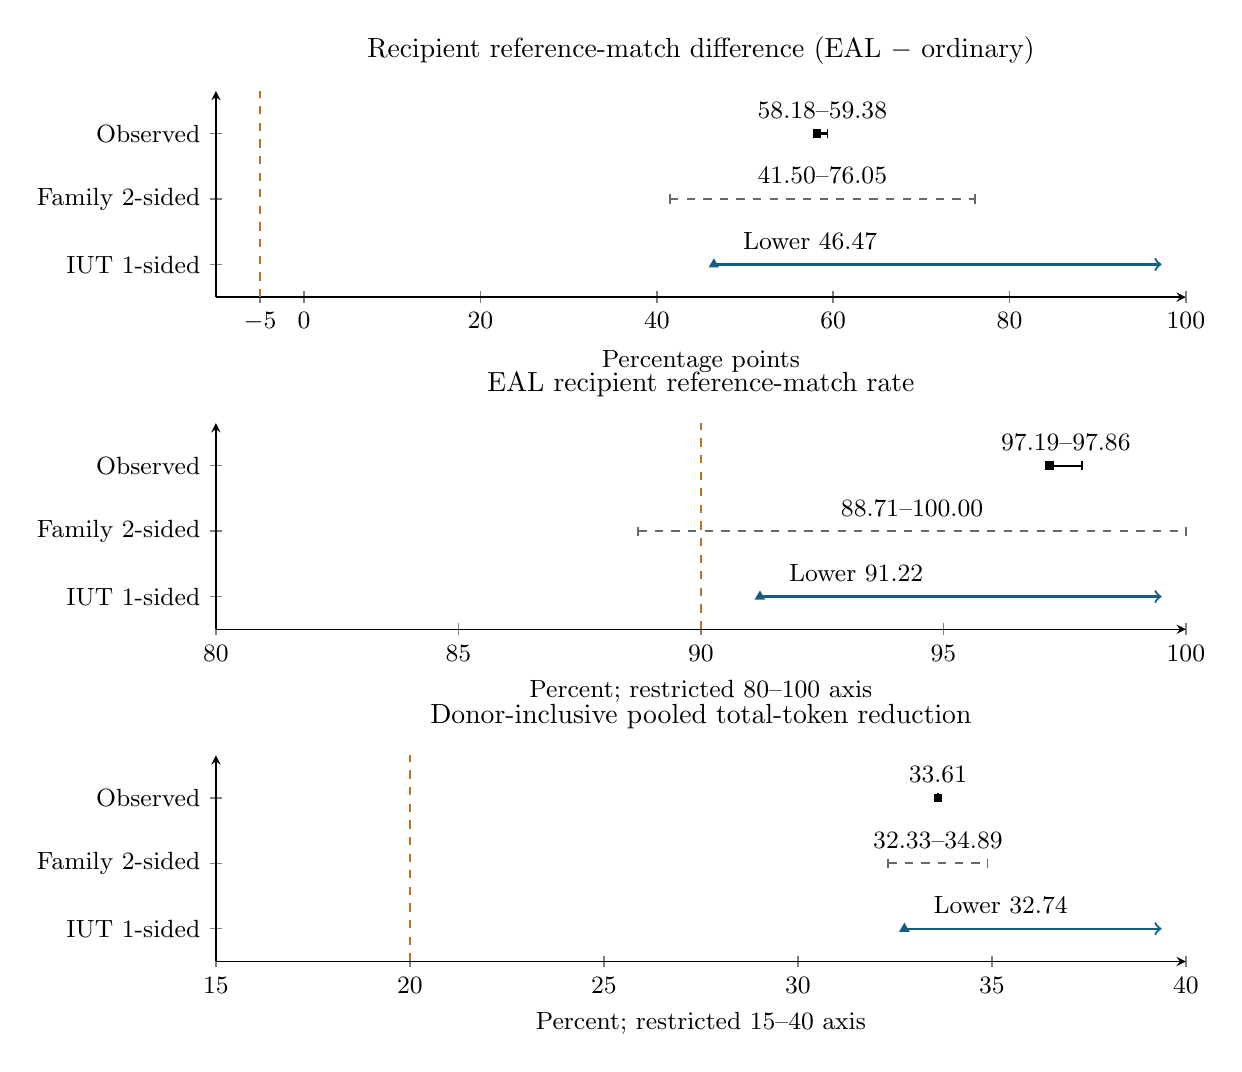
\begin{tikzpicture}
\definecolor{ealblue}{HTML}{165D81}
\definecolor{ordinaryorange}{HTML}{C27021}
\definecolor{neutralgrey}{HTML}{616970}
\pgfplotsset{compat=1.18,
  every axis/.append style={
    width=148mm,height=66mm,
    font=\fontsize{9}{11}\selectfont,
    tick label style={font=\fontsize{9}{11}\selectfont},
    label style={font=\fontsize{9}{11}\selectfont},
    title style={font=\fontsize{10}{12}\selectfont},
    legend style={font=\fontsize{9}{11}\selectfont,draw=none,fill=none},
    axis lines=left,axis line style={line width=0.5pt},
    tick style={line width=0.5pt},
    grid style={line width=0.4pt,black!12},
    scaled ticks=false,clip=false}}
\begin{axis}[name=panel0,width=139mm,height=42mm,xmin=-10,xmax=100,ymin=0.5,ymax=3.65,ytick={1,2,3},yticklabels={IUT 1-sided,Family 2-sided,Observed},xtick={-5,0,20,40,60,80,100},xlabel={Percentage points},title={Recipient reference-match difference (EAL $-$ ordinary)},title style={font=\fontsize{10}{12}\selectfont},axis lines=left]
\addplot[forget plot,ordinaryorange,dashed,line width=0.6pt,no marks] coordinates {(-5,0.5) (-5,3.65)};
\addplot[forget plot,black,solid,line width=0.8pt,no marks] coordinates {(58.17708333,3) (59.375,3)};
\addplot[forget plot,black,line width=0.6pt,no marks] coordinates {(58.17708333,2.93) (58.17708333,3.07)};
\addplot[forget plot,black,line width=0.6pt,no marks] coordinates {(59.375,2.93) (59.375,3.07)};
\addplot[forget plot,black,only marks,mark=square*,mark size=1.3pt,line width=0.5pt] coordinates {(58.17708333,3)};
\node[font=\fontsize{9}{11}\selectfont,anchor=south] at (axis cs:58.77604166666667,3.08) {58.18--59.38};
\addplot[forget plot,neutralgrey,dashed,line width=0.8pt,no marks] coordinates {(41.50402031,2) (76.04806302,2)};
\addplot[forget plot,neutralgrey,line width=0.6pt,no marks] coordinates {(41.50402031,1.93) (41.50402031,2.07)};
\addplot[forget plot,neutralgrey,line width=0.6pt,no marks] coordinates {(76.04806302,1.93) (76.04806302,2.07)};
\node[font=\fontsize{9}{11}\selectfont,anchor=south] at (axis cs:58.77604166666666,2.08) {41.50--76.05};
\addplot[forget plot,ealblue,line width=0.8pt,no marks,->] coordinates {(46.4712601,1) (97.25,1)};
\addplot[forget plot,ealblue,only marks,mark=triangle*,mark size=1.7pt,line width=0.5pt] coordinates {(46.4712601,1)};
\node[font=\fontsize{9}{11}\selectfont,anchor=south west] at (axis cs:48.67126009608052,1.08) {Lower 46.47};
\end{axis}
\begin{axis}[name=panel1,at={(panel0.south west)},yshift=-16mm,anchor=north west,width=139mm,height=42mm,xmin=80,xmax=100,ymin=0.5,ymax=3.65,ytick={1,2,3},yticklabels={IUT 1-sided,Family 2-sided,Observed},xtick={80,85,90,95,100},xlabel={Percent; restricted 80--100 axis},title={EAL recipient reference-match rate},title style={font=\fontsize{10}{12}\selectfont},axis lines=left]
\addplot[forget plot,ordinaryorange,dashed,line width=0.6pt,no marks] coordinates {(90,0.5) (90,3.65)};
\addplot[forget plot,black,solid,line width=0.8pt,no marks] coordinates {(97.1875,3) (97.86458333,3)};
\addplot[forget plot,black,line width=0.6pt,no marks] coordinates {(97.1875,2.93) (97.1875,3.07)};
\addplot[forget plot,black,line width=0.6pt,no marks] coordinates {(97.86458333,2.93) (97.86458333,3.07)};
\addplot[forget plot,black,only marks,mark=square*,mark size=1.3pt,line width=0.5pt] coordinates {(97.1875,3)};
\node[font=\fontsize{9}{11}\selectfont,anchor=south] at (axis cs:97.52604166666666,3.08) {97.19--97.86};
\addplot[forget plot,neutralgrey,dashed,line width=0.8pt,no marks] coordinates {(88.70838264,2) (100,2)};
\addplot[forget plot,neutralgrey,line width=0.6pt,no marks] coordinates {(88.70838264,1.93) (88.70838264,2.07)};
\addplot[forget plot,neutralgrey,line width=0.6pt,no marks] coordinates {(100,1.93) (100,2.07)};
\node[font=\fontsize{9}{11}\selectfont,anchor=south] at (axis cs:94.35419132225901,2.08) {88.71--100.00};
\addplot[forget plot,ealblue,line width=0.8pt,no marks,->] coordinates {(91.21760934,1) (99.5,1)};
\addplot[forget plot,ealblue,only marks,mark=triangle*,mark size=1.7pt,line width=0.5pt] coordinates {(91.21760934,1)};
\node[font=\fontsize{9}{11}\selectfont,anchor=south west] at (axis cs:91.61760934305097,1.08) {Lower 91.22};
\end{axis}
\begin{axis}[name=panel2,at={(panel1.south west)},yshift=-16mm,anchor=north west,width=139mm,height=42mm,xmin=15,xmax=40,ymin=0.5,ymax=3.65,ytick={1,2,3},yticklabels={IUT 1-sided,Family 2-sided,Observed},xtick={15,20,25,30,35,40},xlabel={Percent; restricted 15--40 axis},title={Donor-inclusive pooled total-token reduction},title style={font=\fontsize{10}{12}\selectfont},axis lines=left]
\addplot[forget plot,ordinaryorange,dashed,line width=0.6pt,no marks] coordinates {(20,0.5) (20,3.65)};
\addplot[forget plot,black,solid,line width=0.8pt,no marks] coordinates {(33.60920874,3) (33.60920874,3)};
\addplot[forget plot,black,line width=0.6pt,no marks] coordinates {(33.60920874,2.93) (33.60920874,3.07)};
\addplot[forget plot,black,line width=0.6pt,no marks] coordinates {(33.60920874,2.93) (33.60920874,3.07)};
\addplot[forget plot,black,only marks,mark=square*,mark size=1.3pt,line width=0.5pt] coordinates {(33.60920874,3)};
\node[font=\fontsize{9}{11}\selectfont,anchor=south] at (axis cs:33.60920873730253,3.08) {33.61};
\addplot[forget plot,neutralgrey,dashed,line width=0.8pt,no marks] coordinates {(32.32777348,2) (34.890644,2)};
\addplot[forget plot,neutralgrey,line width=0.6pt,no marks] coordinates {(32.32777348,1.93) (32.32777348,2.07)};
\addplot[forget plot,neutralgrey,line width=0.6pt,no marks] coordinates {(34.890644,1.93) (34.890644,2.07)};
\node[font=\fontsize{9}{11}\selectfont,anchor=south] at (axis cs:33.60920873730253,2.08) {32.33--34.89};
\addplot[forget plot,ealblue,line width=0.8pt,no marks,->] coordinates {(32.74494073,1) (39.375,1)};
\addplot[forget plot,ealblue,only marks,mark=triangle*,mark size=1.7pt,line width=0.5pt] coordinates {(32.74494073,1)};
\node[font=\fontsize{9}{11}\selectfont,anchor=south west] at (axis cs:33.24494073397548,1.08) {Lower 32.74};
\end{axis}
\end{tikzpicture}
